\documentclass{report}
\usepackage{float}

% for the image in the title
\usepackage{tikz}

% custom spacing
\usepackage{setspace}
\onehalfspacing

% footer and header
\usepackage{fancyhdr}
% \setlength{\headheight}{15.2pt}

% underlining
\usepackage{ulem}


% Table of contents link to corresponding sections
\usepackage{hyperref}
\hypersetup{
	colorlinks,
	citecolor=black,
	filecolor=black,
	linkcolor=black,
	urlcolor=black
}

\usepackage{amsmath}
% Remove che "Chapter" string before chapters
\iffalse
\makeatletter
\def\@makechapterhead#1{%
	\vspace*{50\p@}%
	{\parindent \z@ \raggedright \normalfont
		\interlinepenalty\@M
		\Huge\bfseries  \thechapter.\quad #1\par\nobreak
		\vskip 40\p@
}}
\makeatother
\fi

% Fancy chapters
\usepackage[Bjarne]{fncychap}
% options: Sonny, Lenny, Glenn, Conny, Rejne, Bjarne, Bjornstrup

\begin{document}
	
	
	%title page
	\begin{titlepage}
		\begin{figure}[t]
			\centering
\includegraphics[width=0.3\textwidth]{images/unitn-logo}
		\end{figure}
		\begin{center}
			\textsc{ \LARGE{Università degli Studi di Trento \\}}
			\textsc{ \LARGE{Facoltà di Informatica\\ }}
			\textnormal{ \LARGE{Corso di Ingegneria del Software\\}}
			\vspace{30mm}
			\fontsize{10mm}{7mm}\selectfont 
			\textup{Fix Mi \\ Application Implementation and Documentation}\\
		\end{center}
		
		\vspace{25mm}
		
		\centering
		\large Gruppo G43: \\ Giovanni Santini\\ Riginel Ungureanu \\ Valerio Asaro
		
		\vspace{20mm}
		
		\centering{\large{Anno Accademico 2023/2024 \\ Trento }}
		
	\end{titlepage}
	
	
	
	
	% use header and footers
	\pagestyle{fancy}
	\fancyhead[R]{\chaptername\ \thechapter}  % header
	
	%\maketitle
	\tableofcontents
	\newpage
	
	
	
	\section{Scopo del documento}
	
	
	\section{Implementazione}
	
	\section{Informazioni del Documento}
	
	% table
	\begin{center} % center the table
		\centering
		\begin{tabular}{ |p{4cm}|p{4cm}|  }
			\hline
			\centering Campo & \qquad\qquad Valore \\ % I found no other way...
			\hline
			Titolo del Documento & Application Implementation and Documentation \\
			\hline
			Titolo del Progetto & Fix Mi \\
			\hline
			Autori del Documento &
			Giovanni Santini \\ & Riginel Ungureanu \\ & Valerio Asaro \\
			\hline
			Amministratore Progetto & Riginel Ungureanu\\
			\hline
			Versione del documento & 1.0 \\
			\hline
		\end{tabular}
	\end{center}
	
	
	
\chapter{Backend}

Il seguente capitolo descrive l'implementazione, con il supporto di diagrammi "UML" e codice, della parte "Backend" dell'applicazione, in riferimento a quanto detto nei precedenti documenti quali "Analisi dei Requisiti", "Specifica dei Requisiti" e del "Documento di Architettura".  Il capitolo è strutturato partendo da una visione generale dell'infrastruttura, andando verso una visione più specifica e dettagliata.


Gli estratti di codice verranno mostrati nel seguente formato:
\begin{figure}[H]
	\centering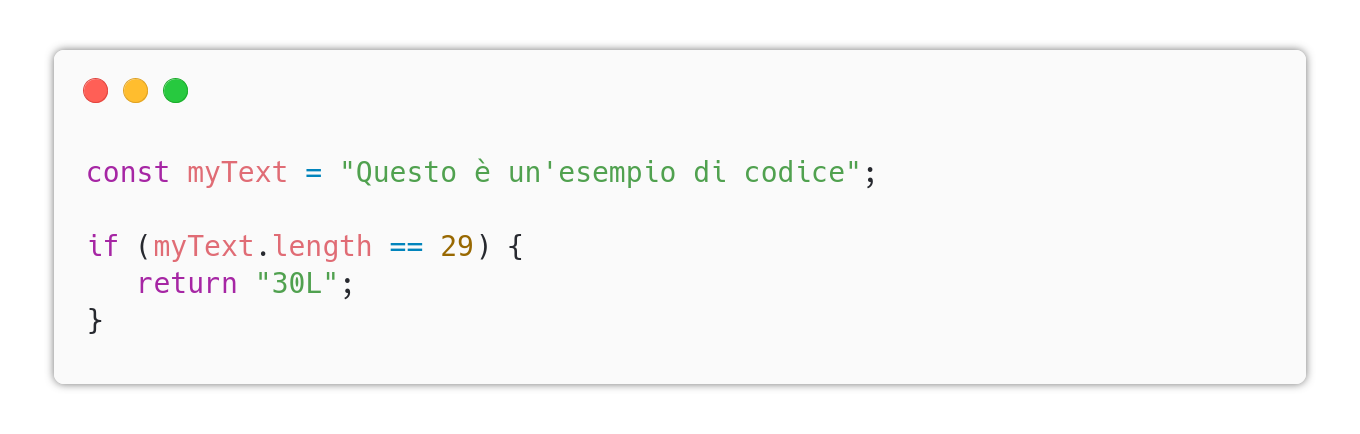
\includegraphics[width=1\textwidth]{images/example_code_01.png}
	Esempio di estratto di codice
\end{figure}

\subsection*{Tecnologie}

In questo capitolo verranno menzionate più volte alcune tecnologie, dunque ne viene riportata una breve descrizionee sotto:
\begin{itemize}
	\item "Docker": tecnologia che raccoglie il software in unità standardizzate chiamate container, offrendo tutto il necessario per la loro corretta esecuzione, incluse librerie, strumenti di sistema, codice e runtime. Il logo ricorda una balena di colore azzurro con dei rettangoli al di sopra rappresentanti dei containers, come se la balena stessa fosse una nave.
	\item "Docker Compose": software per la gestione di molteplici docker containers contemporaneamente. L'icona rappresenta un polpo con dei parallelepipedi azzurri tra i tentacoli.
	\item "Nginx": intermediario tra le richieste da parte dei client e il server. Può essere usato come load balancer, cache o proxy. Il logo è raffigurato da un N bianca con sfondo verde.
	\item "MongoDB": DBMS non relazionale. Il logo rappresenta una foglia verde.
	\item "Express": framework backend per applicazioni web in javascript. Il logo è formato dalle due lettere "e" e "x" in nero.
	\item "React": framework frontend lo sviluppo di applicazioni web. L'icona ricorda un atomo.
\end{itemize}

\section{Architettura dei Microservizi}

L'architettura proposta si basa sulla divisione logica (e fisica) delle funzionalità dell'applicazione tramite la distinzione di \textit{Microservizi}. Ciascun microservizio è indipendente dagli altri ed è composto a sua volta da una frontend e una backend distinte. Per tale ragione, è più accurato parlare di micro-frontend e micro-backend.

\subsection*{Vantaggi di un'architettura basata su microservizi}

Da un punto di vista di sviluppo, un'architettura non monolitica permette lo sviluppo asincrono dei singoli microservizi, oltre a facilitare la divisione del lavoro nelle varie parti. Tale architettura ha anche dei vantaggi a livello di performance in quanto il carico di lavoro chel'applicazione processa viene distribuito su più processi diminuendo il carico sul singolo. Altri vantaggi sono la scalarità dia una componente dell'applicazione in base alle esigenze e la ridondanza in quanto possono esistere più istanze di un microservizio contemporaneamente.

\subsection*{Svantaggi}

Un'architettura a microservizi è intrinsecamente più complessa nella progettazzione e nella menutenzione rispetto ad una architettura tradizionale. La necessità di orchestrare e mettere in comunicazione i diversi microservizi richiede particolari accortezze nella parte di design e di deploy. Tali problematiche sono state valutate con cura dal team di sviluppo.

\section{Visione Generale}
Prima di analizzare il singolo microservizio, questa sezione illustra una visione generale dell'applicazione e degli strumenti utilizzati per la realizzazione dell'infrastruttura, per poi concentrarsi sulle parti comuni di ogni microservizio e infine sul singolo microservizio.


\subsection*{Infrastruttura}

Si presti attenzione alla seguente infografica dell'infrastruttura implementata:

\begin{figure}[H]
	\centering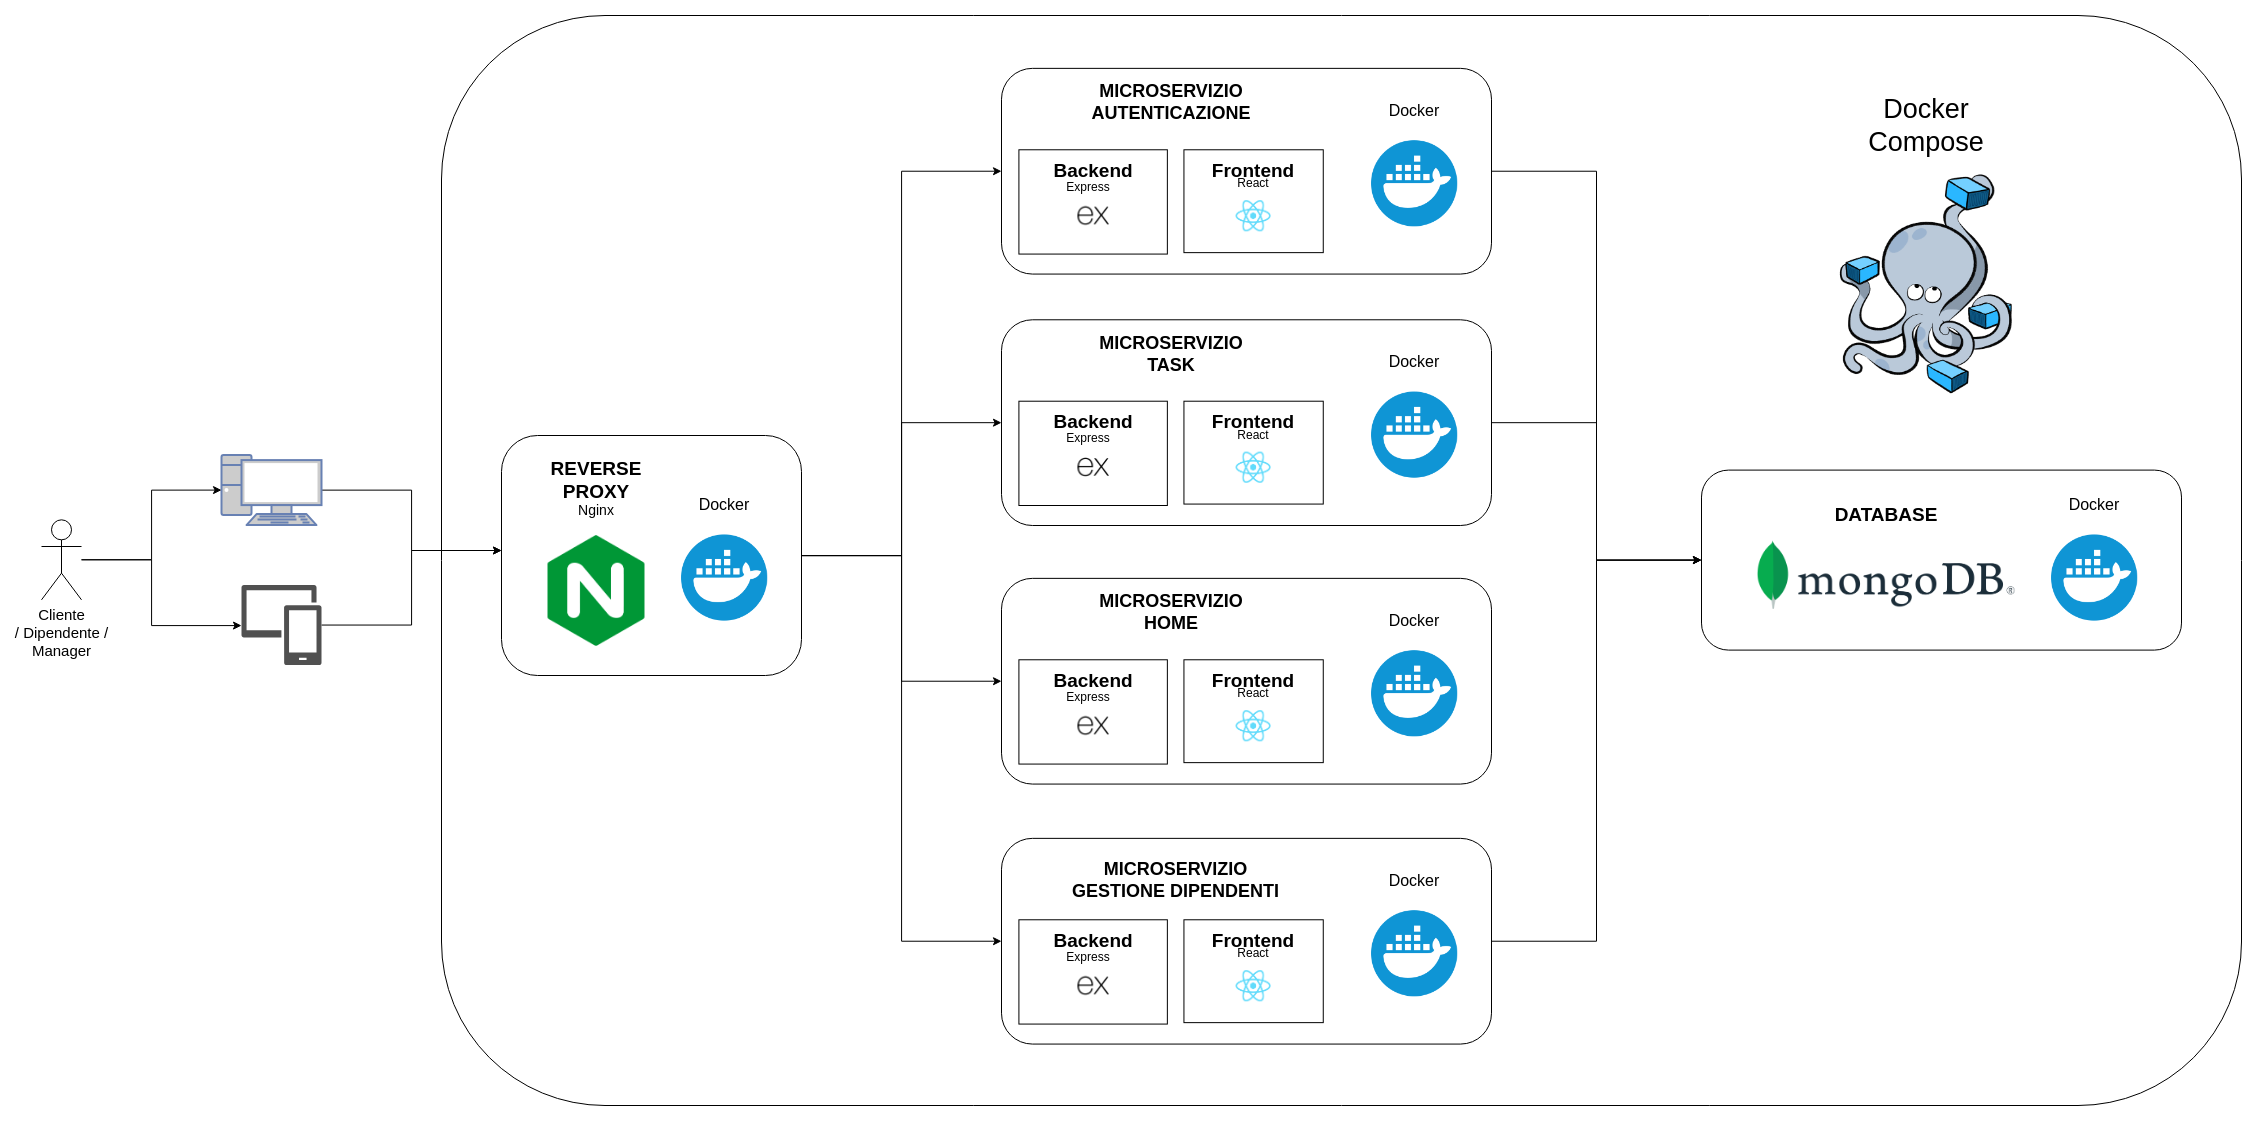
\includegraphics[width=1\textwidth]{images/diagramma_microservizi.png}
	Schema dei microservizi
\end{figure}

L'intera infrastruttura viene inizializzata con \textit{Docker Compose}. In particolare, \textit{Docker Compose} si occupa di impostare i containers sullo stesso network con un IP statico e le variabili di ambiente come le porte e gli IP dei rispettivi microservizi, oltre ad inizializzare i containers, le porte e volumi condivisi.

Se eseguito su un singolo host, il network di default segue la seguente struttura:
\begin{figure}[H]
	\centering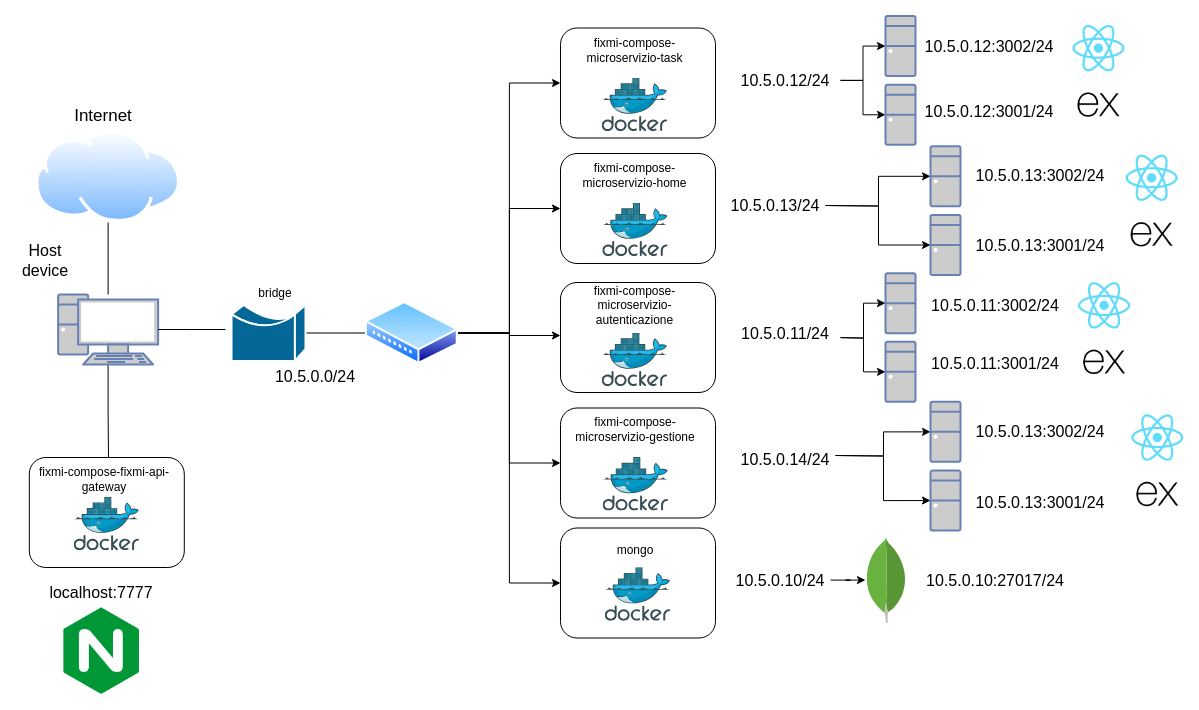
\includegraphics[width=1\textwidth]{images/network.png}
	Schema del network dei microservizi
\end{figure}

Docker imposta i microservizi sul network 10.5.0.0/24 con i seguenti IP:
	% table
\begin{center} % center the table
	\centering
	\begin{tabular}{ |p{4cm}|p{4cm}|  }
		\hline
		\centering Nome Microservizio & \qquad\quad Network IP \\ % I found no other way...
		\hline
		MongoDB & 10.5.0.10/24 \\
		\hline
		Microservizio Autenticazione & 10.5.0.11/24 \\
		\hline
		Microservizio Task & 10.5.0.12/24 \\
		\hline
		Microservizio Home & 10.5.0.13/24 \\
		\hline
		Microservizio Gestione Dipendenti & 10.5.0.14/24 \\
		\hline
		Reverse Proxy & 127.0.0.1 \\
		\hline
	\end{tabular}
\end{center}

Ad ogni servizio sono state assegnate le seguenti porte:

\begin{center} % center the table
	\centering
	\begin{tabular}{ |p{4cm}|p{4cm}|  }
		\hline
		\centering Nome servizio & \qquad\qquad Porta \\ % I found no other way...
		\hline
		MongoDB & 27017 \\
		\hline
		Backend & 3001 \\
		\hline
		frontend & 3002 \\
		\hline
		Reverse Proxy & 7777 \\
		\hline
	\end{tabular}
\end{center}

Due microservizi particolari sono il database e il reverse proxy. Il database fornisce la possibilità di salvare in modo permanente i dati dell'applicazione, mentre il reverse proxy permette di accedere facilmente all'ip di un microservizio attraverso una mappatura di ip. I software scelti sono rispettivamente \textit{MongoDB} e \textit{Nginx}.

In particolare, \textit{Nginx} associa le routes nel seguente modo:
\begin{figure}[H]
	\centering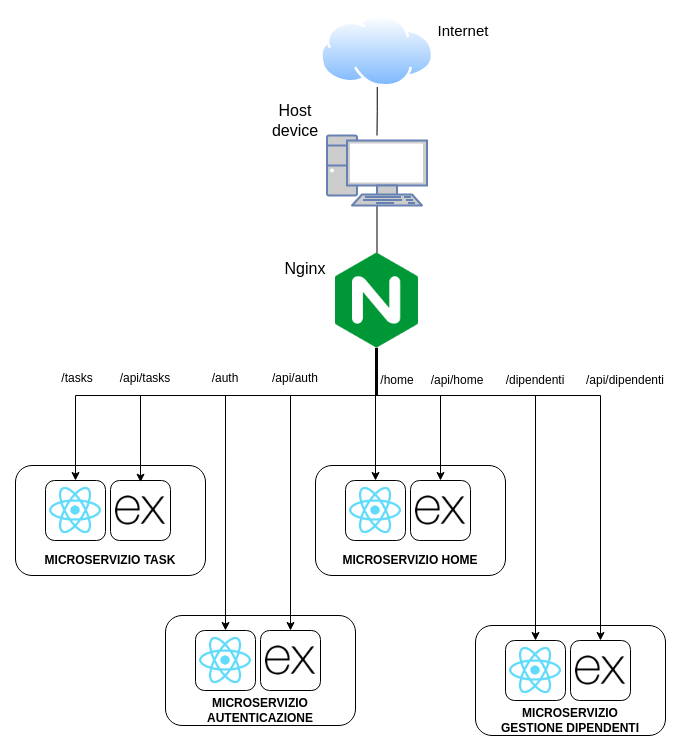
\includegraphics[width=1\textwidth]{images/nginx.png}
	Schema delle routes di Nginx
\end{figure}

\subsection*{Codice: Struttura}

La directory radice del progetto contiene i seguenti files:

\begin{figure}[H]
	\centering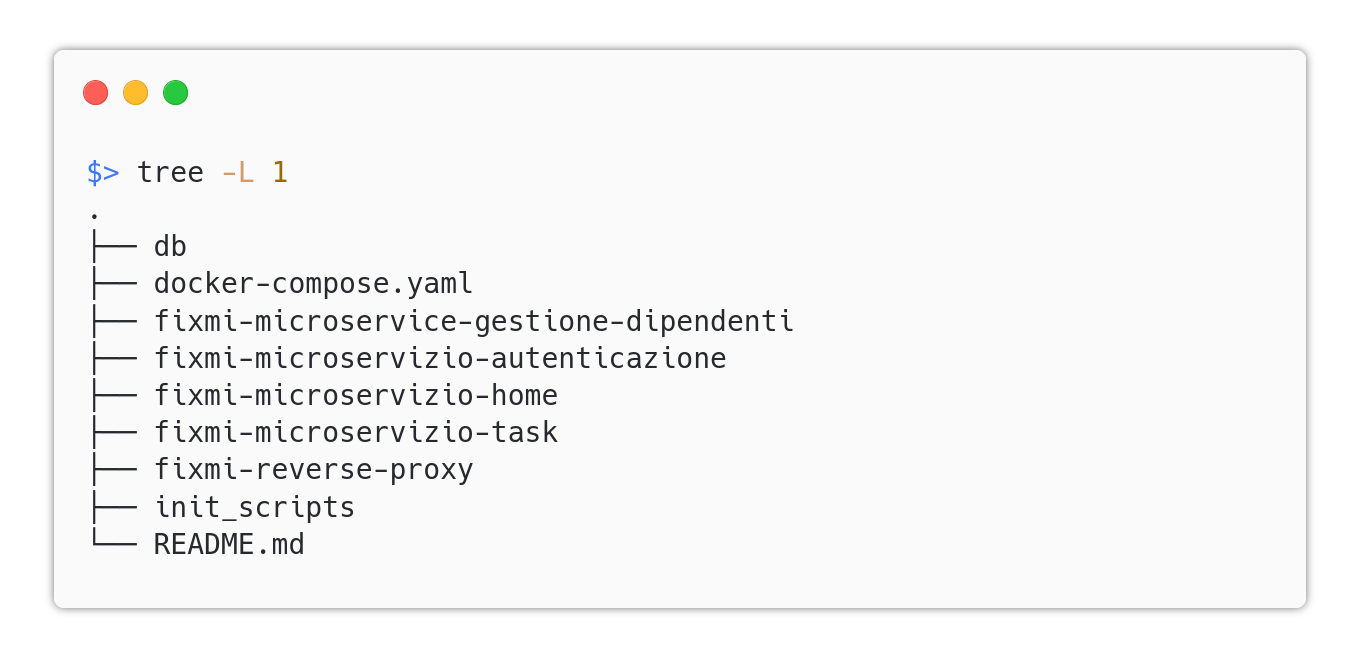
\includegraphics[width=1\textwidth]{images/tree.png}
    Output del comando "tree", mostra i contenuti della directory root del progetto.
\end{figure}

Segue una descrizione degli stessi:
\begin{itemize}
	\item "db": volume condiviso tra il docker container del database e il filesystem dell'host per mantenere persistenza dei dati quando il container viene riavviato o rimosso.
	\item "docker-compose.yaml": file di configurazione utilizzato da docker compose per inizializzare l'infrastruttura. Contiene le informazioni per avviare gli altri microservizi.
	\item "fixmi-microservice-gestione-dipendenti": cartella contenente il microservizio "Gestione Dipendenti".
	\item "fixmi-microservizio-autenticazione": cartella contenente il microservizio "Autenticazione".
	\item "fixmi-microservizio-home": cartella contenente il microservizio "Home".
	\item "fixmi-microservizio-task": cartella contenente il microservizio "task".
	\item "fixmi-reverse-proxy": cartella contenente il reverse proxy.
	\item "init\_scripts": script per inizializzare il database con dei dati di esempio.
	\item "README.md": contiene informazioni e documentazione sul deploy dell'infrastruttura.
\end{itemize}

\subsection*{Codice: docker-compose.yaml}

Si prenda come esempio questo frammento di codice responsabile del setup del microservizio task:
\begin{figure}[H]
	\centering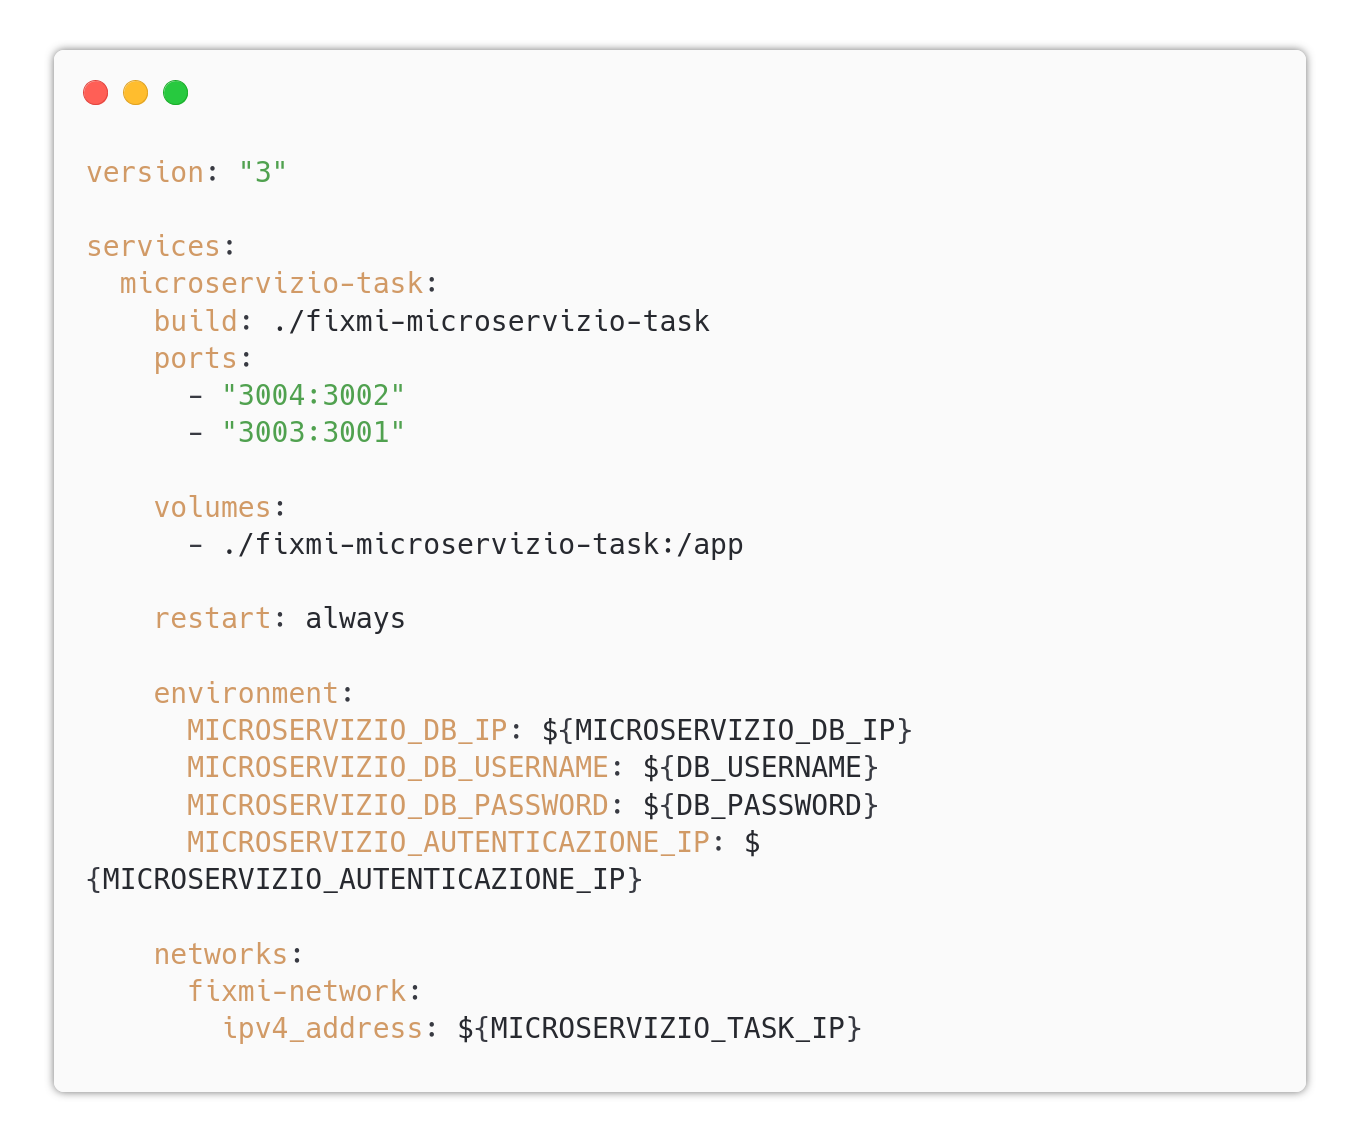
\includegraphics[width=1\textwidth]{images/docker_code_01.png}
	Estratto dal file "docker-compose.yaml"
\end{figure}

In questo codice, notiamo che le porte vengono impostate sotto la sezione "ports", così come i volumi e il network. Le variabili d'ambiente contenenti i vari ip e le credenziali del database sono contenute nel file ".env" presente nella radice della cartella.
La configurazione per gli altri microservizi è simile, con qualche piccola differenza. Qua sotto vengono riportati gli altri microservizi:
\begin{figure}[H]
	\centering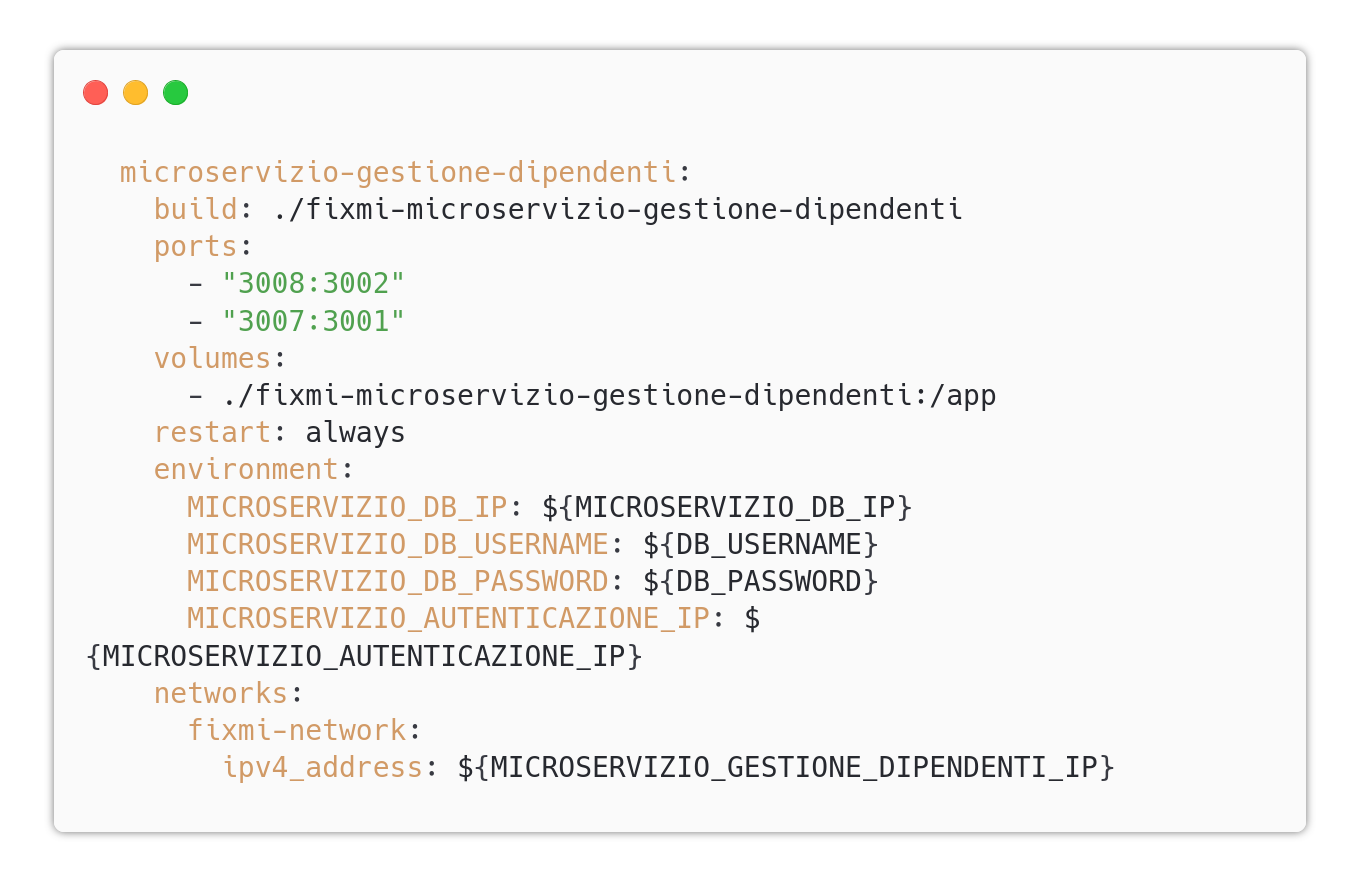
\includegraphics[width=1\textwidth]{images/yaml_gestione_dipendenti.png}
	Codice responsabile per l'avvio del microservizio "Gestione Dipendenti"
\end{figure}
\begin{figure}[H]
	\centering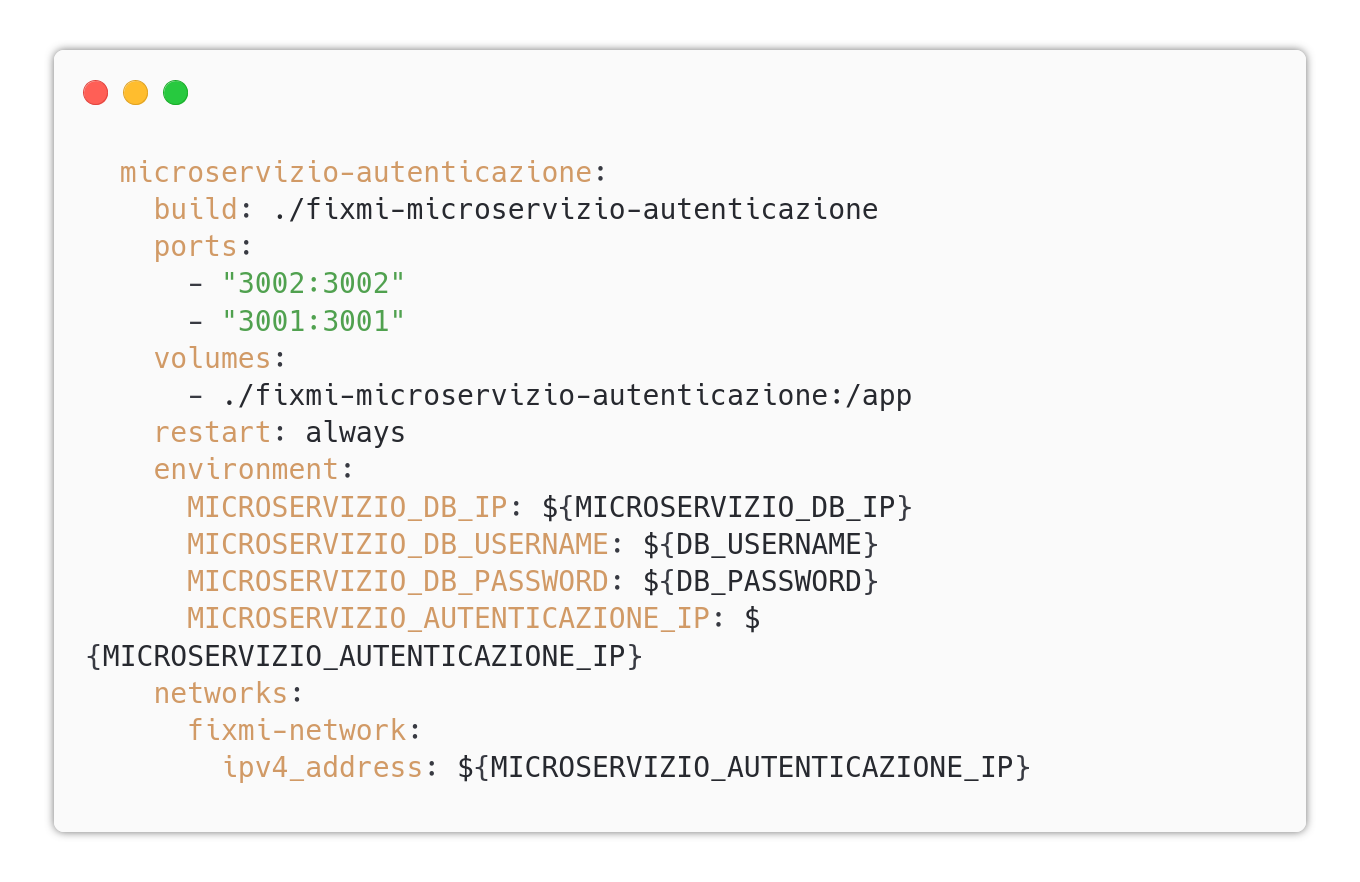
\includegraphics[width=1\textwidth]{images/yaml_autenticazione.png}
	Codice responsabile per l'avvio del microservizio "Autenticazione"
\end{figure}
\begin{figure}[H]
	\centering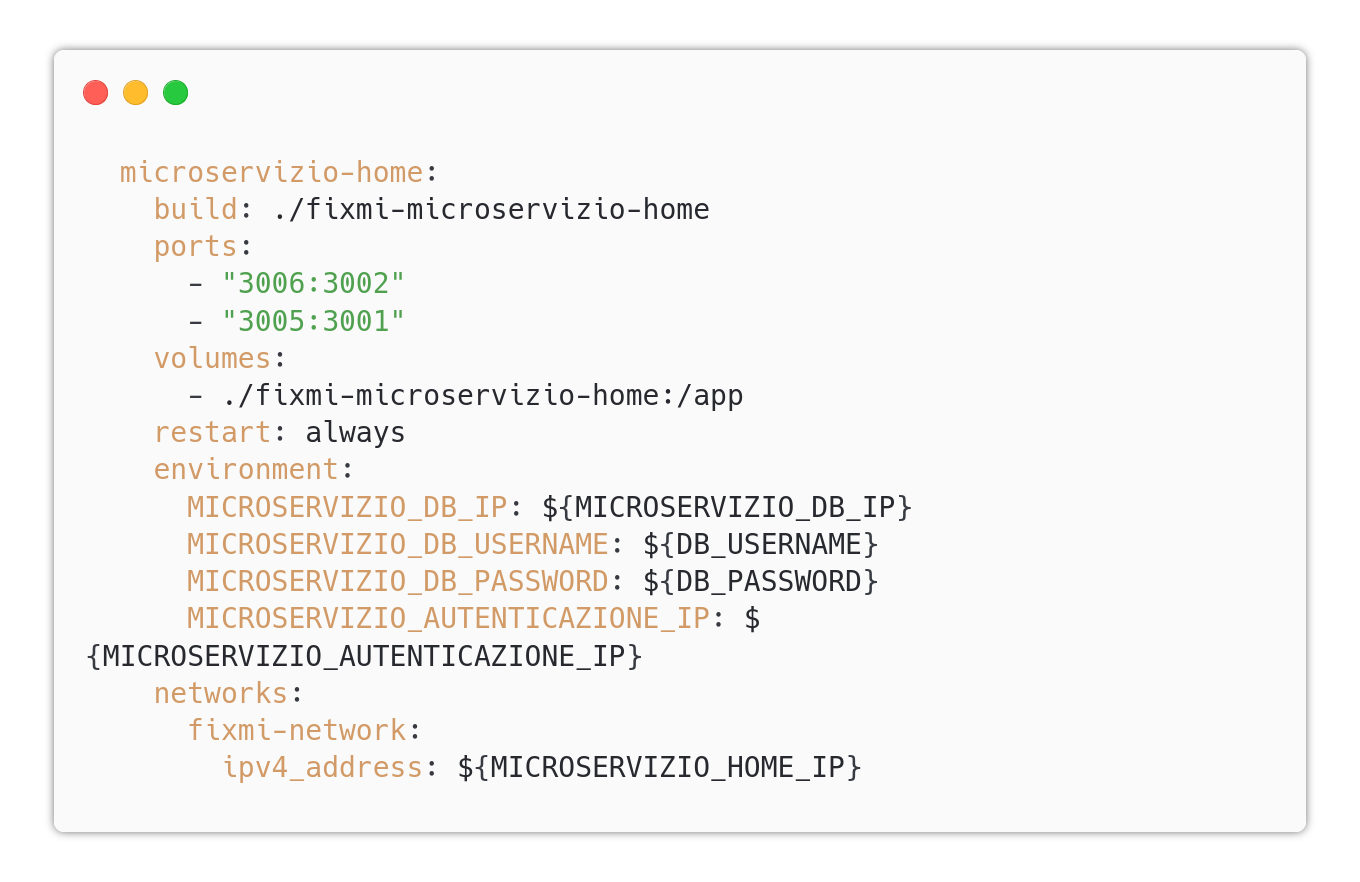
\includegraphics[width=1\textwidth]{images/yaml_home.png}
	Codice responsabile per l'avvio del microservizio "Home"
\end{figure}
\begin{figure}[H]
	\centering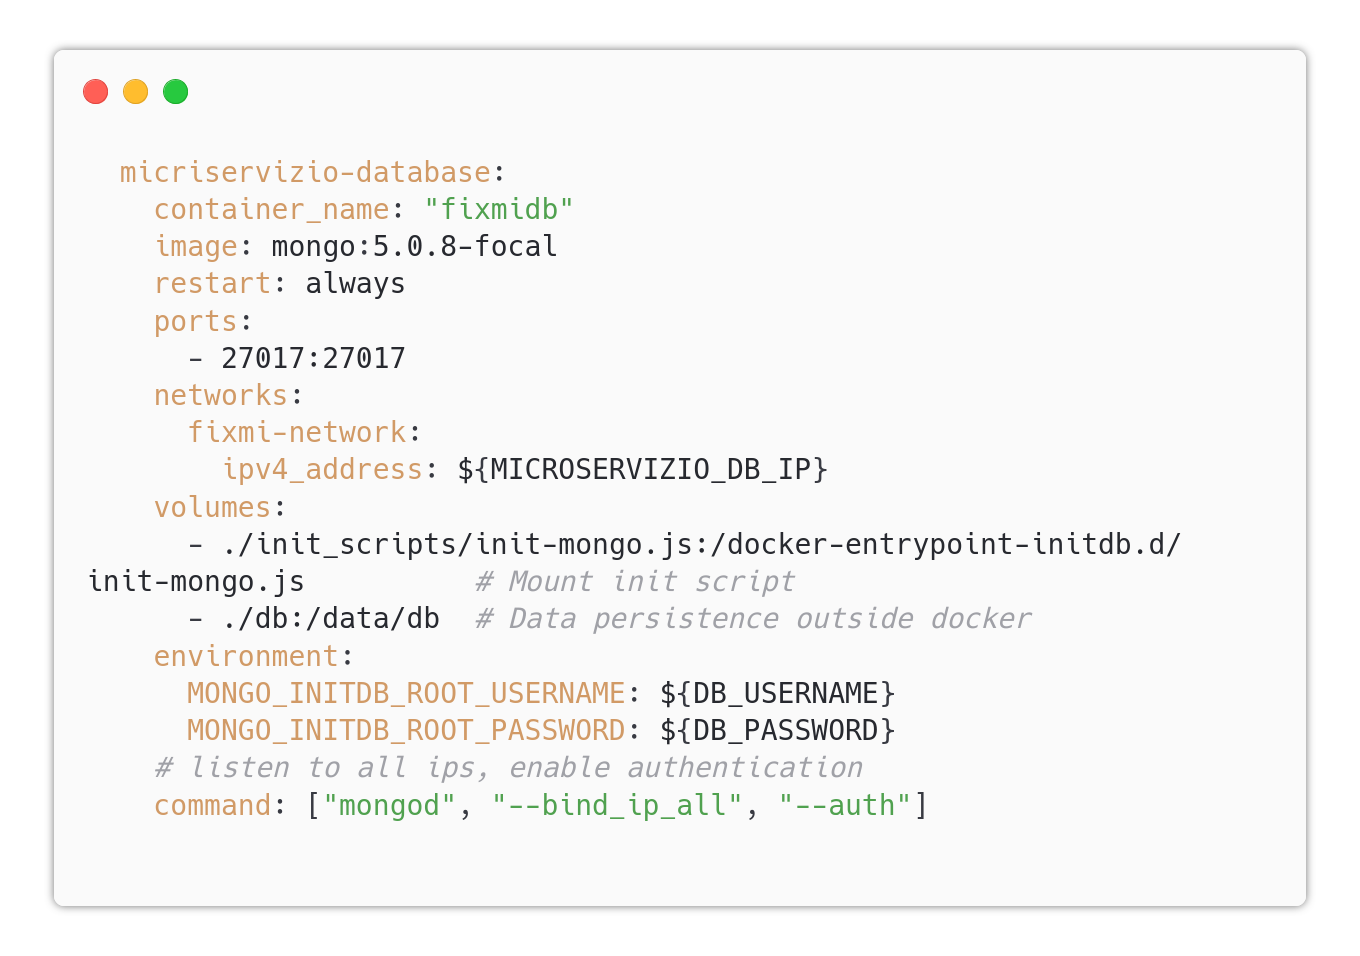
\includegraphics[width=1\textwidth]{images/yaml_database.png}
	Codice responsabile per l'avvio del database
\end{figure}
\begin{figure}[H]
	\centering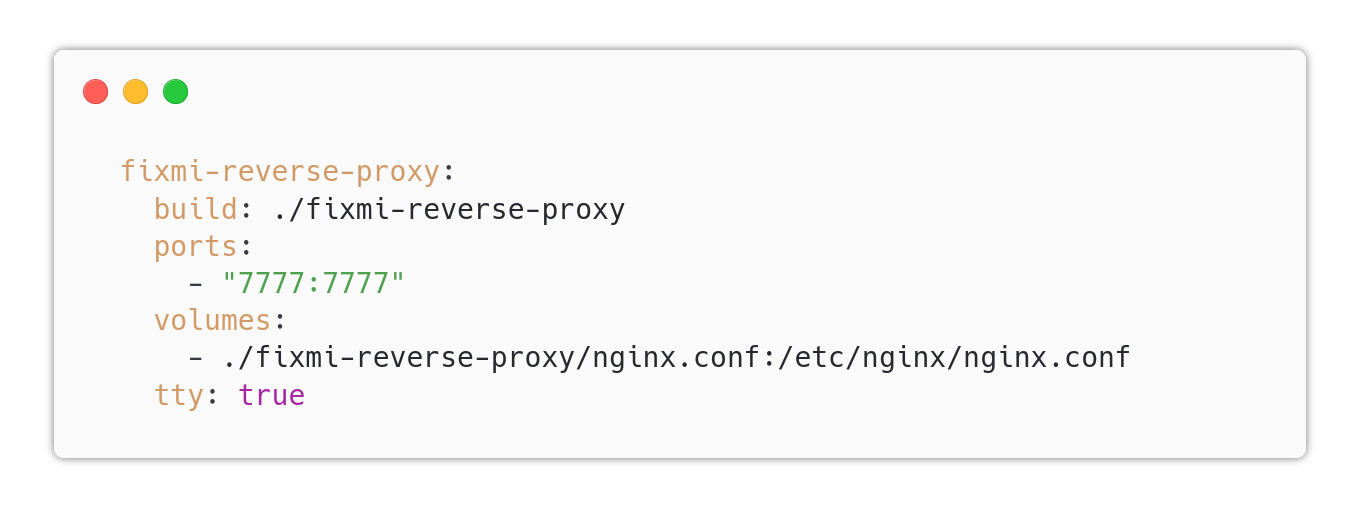
\includegraphics[width=1\textwidth]{images/yaml_reverse_proxy.png}
	Codice responsabile per l'avvio del reverse proxy
\end{figure}

\subsection*{Codice: nginx.conf}

Il file \textit{nginx.conf} all'interno della cartella \textit{fixmi-reverse-proxy} imposta la configurazione per il reverse proxy. Questo microservizio si occupa di instradare le richieste ai vari microservizi. Segue un'estratto della configurazione:


\begin{figure}[H]
	\centering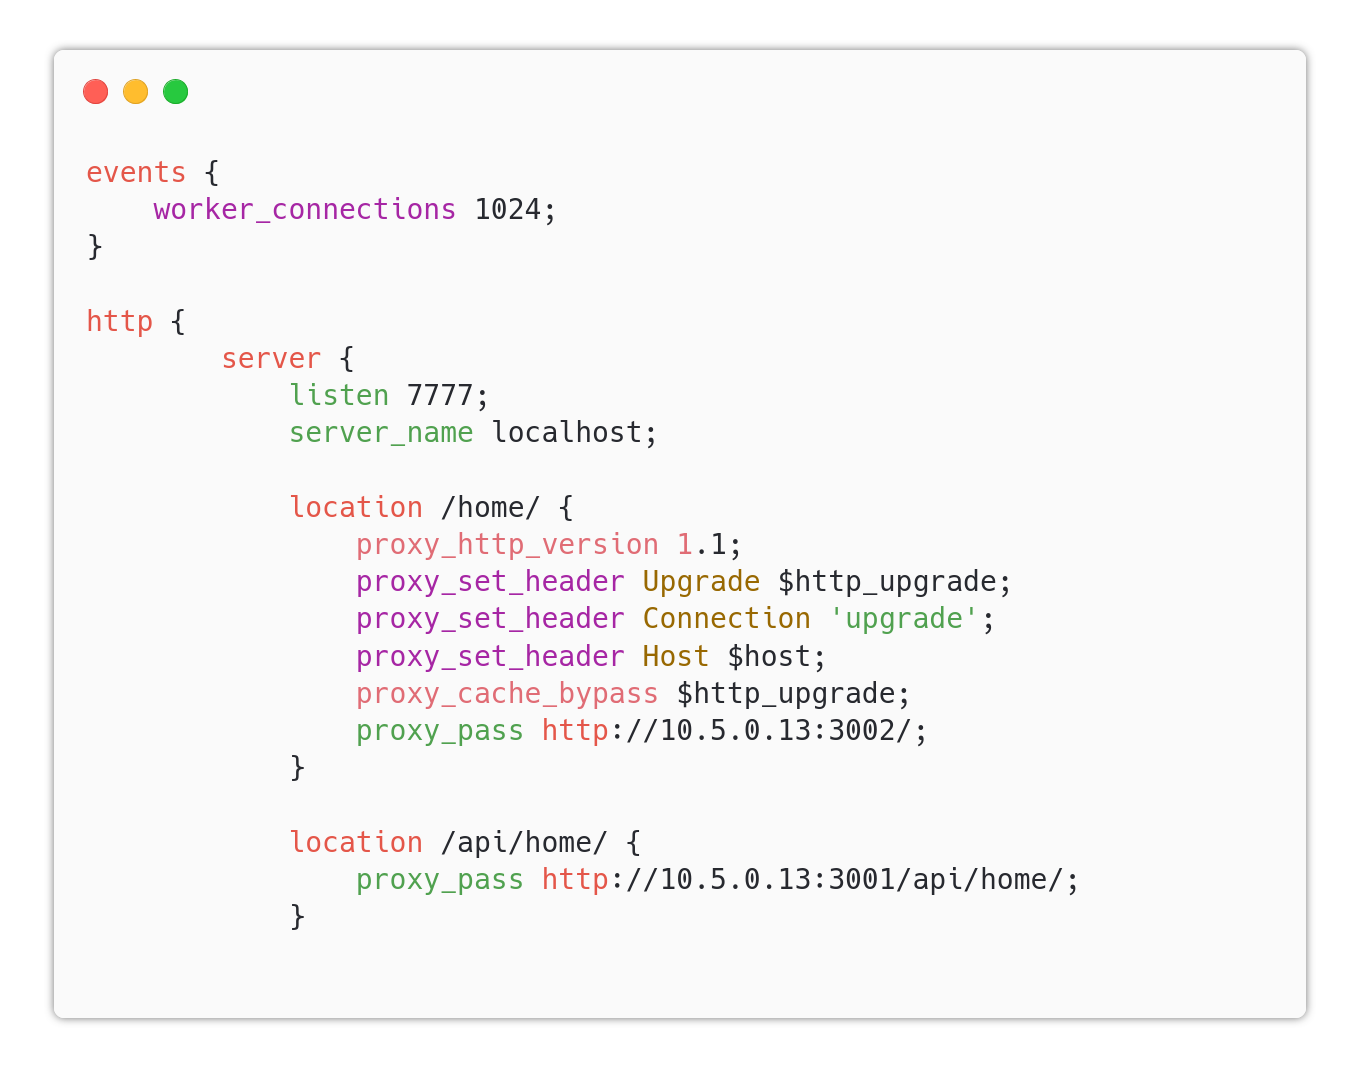
\includegraphics[width=1\textwidth]{images/nginx_config_home.png}
	Estratto da "fixmi-reverse-proxy/nginx.conf", definizione delle routes "/home" e "/api/home"
\end{figure}

La variabile "worker\_connections" definisce il numero di connessioni simultanee che il servizio può gestire. Il blocco "http" e il blocco "server" contengono le configurazioni delle routes, in particolare in questo esempio notiamo che la route "/home/" viene passata a "http://10.5.0.13:3002/" ossia la frontend del microservizio "home", mentre "/api/home/" rimanda a "http://10.5.0.13:3001/api/home/" ossia la backend del microservizio "home". Vengono inoltre impostati alcuni headers dopo la dicitura "proxy\_set\_header".

Di seguito vengono riportate le altre routes:

\begin{figure}[H]
	\centering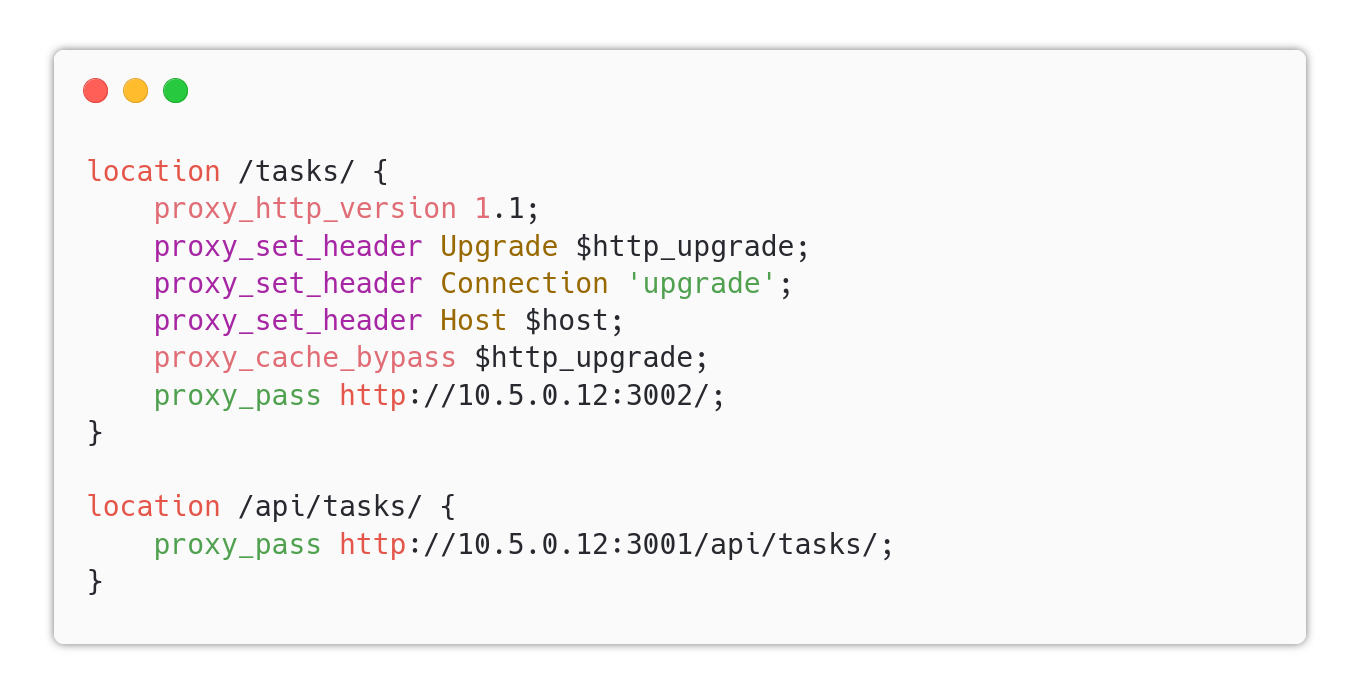
\includegraphics[width=1\textwidth]{images/nginx_config_tasks.png}
	Routes "/tasks" e "/api/tasks"
\end{figure}
\begin{figure}[H]
	\centering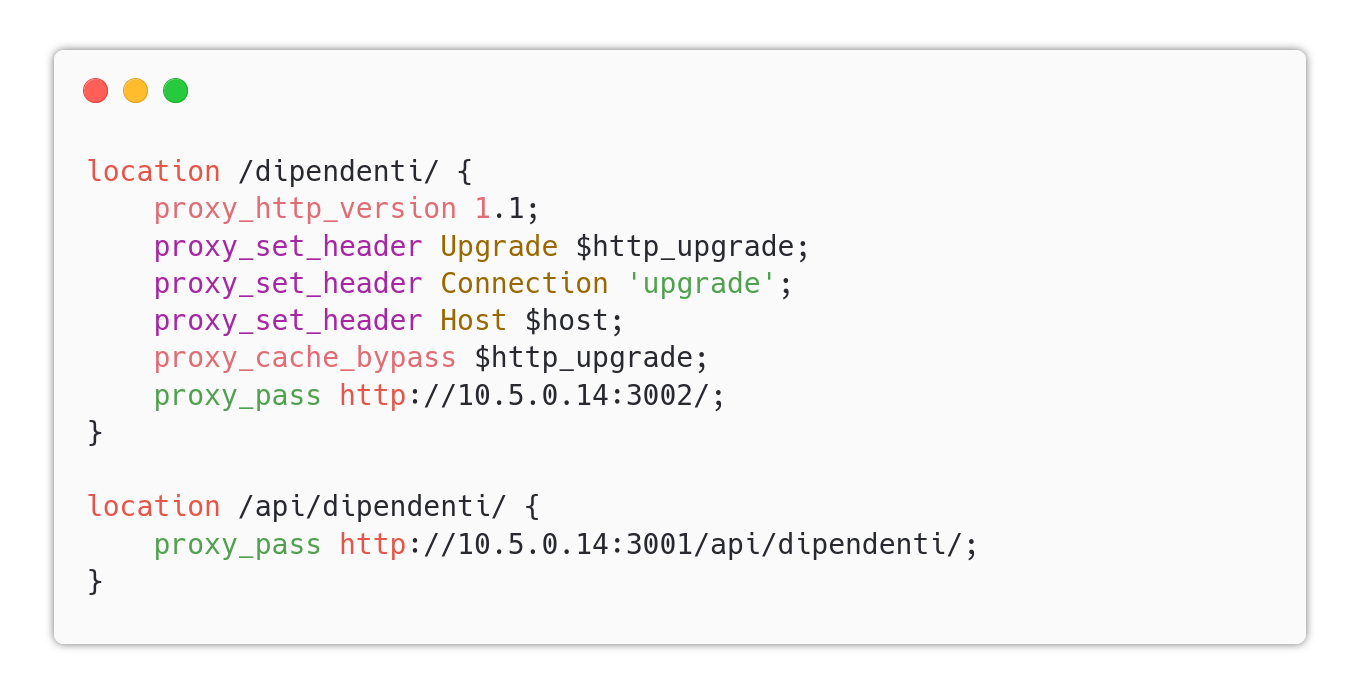
\includegraphics[width=1\textwidth]{images/nginx_config_dipendenti.png}
	Routes "/dipendenti" e "/api/dipendenti"
\end{figure}
\begin{figure}[H]
	\centering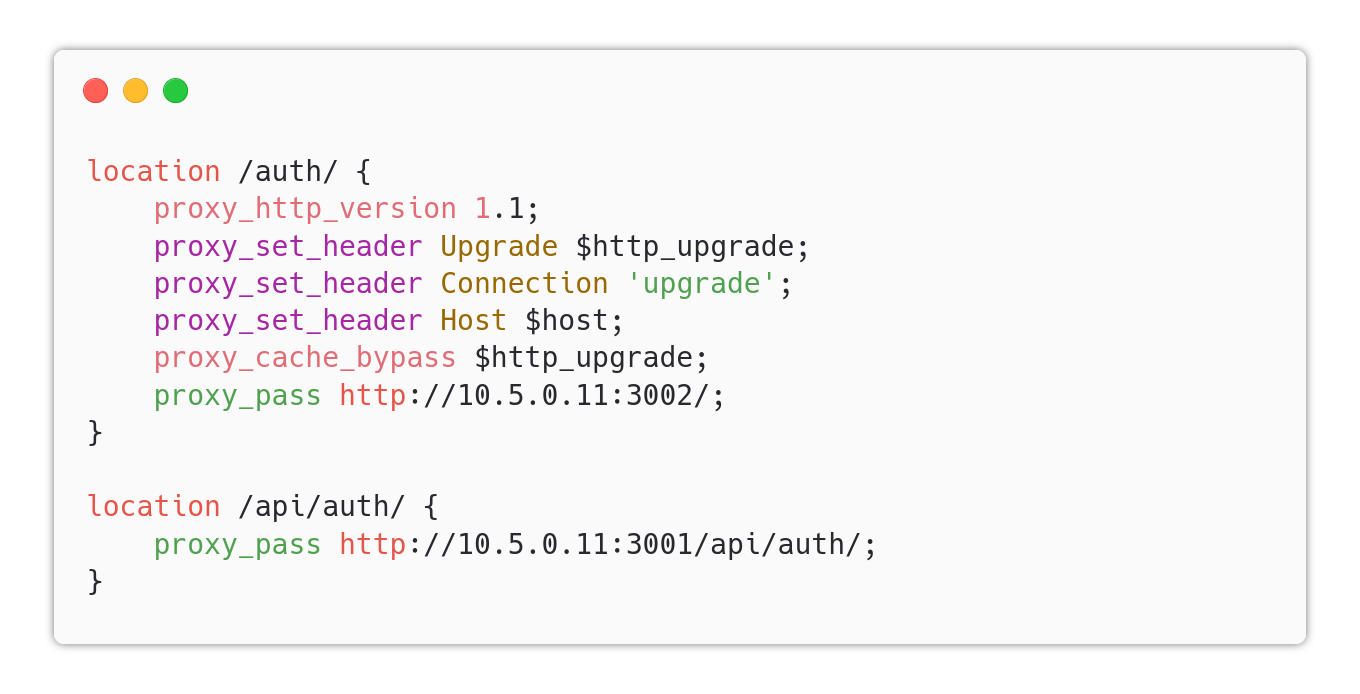
\includegraphics[width=1\textwidth]{images/nginx_config_auth.png}
	Routes "/auth" e "/api/auth"
\end{figure}

\subsection*{Codice: init-mongo.js}

Il file contiene l'inizializzazione delle entrate del database in formato json. Sono stati individuati due database: "Tasks" e "Users" e le rispettive collezioni "tasks" e "users" (da notare la differenza della prima lettera da maiuscola a minuscola). I contenuti sono i seguenti:
\begin{figure}[H]
	\centering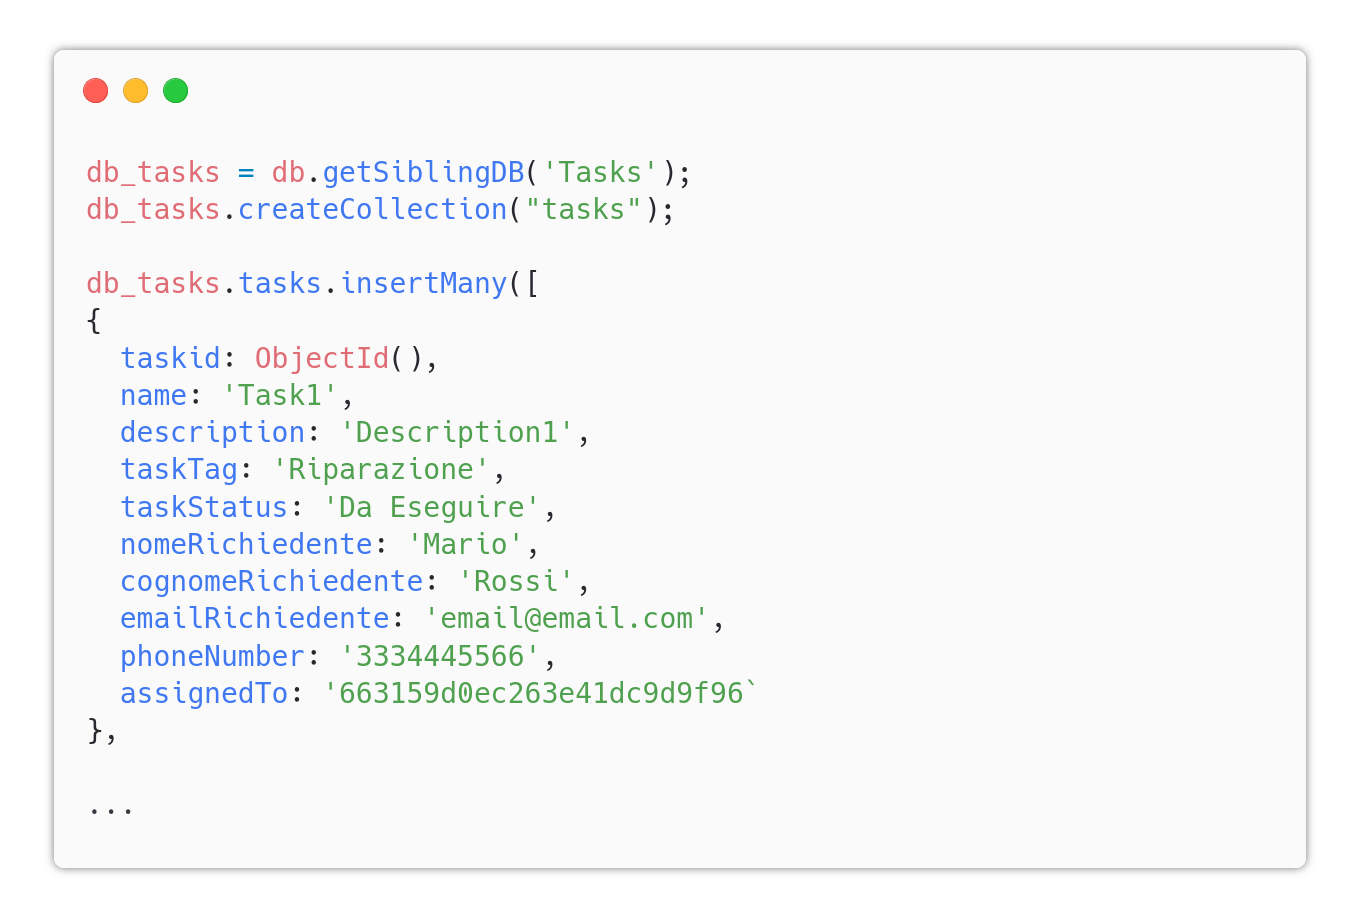
\includegraphics[width=1\textwidth]{images/db-tasks.png}
	Inizializzazione database "Task"
\end{figure}

\begin{figure}[H]
	\centering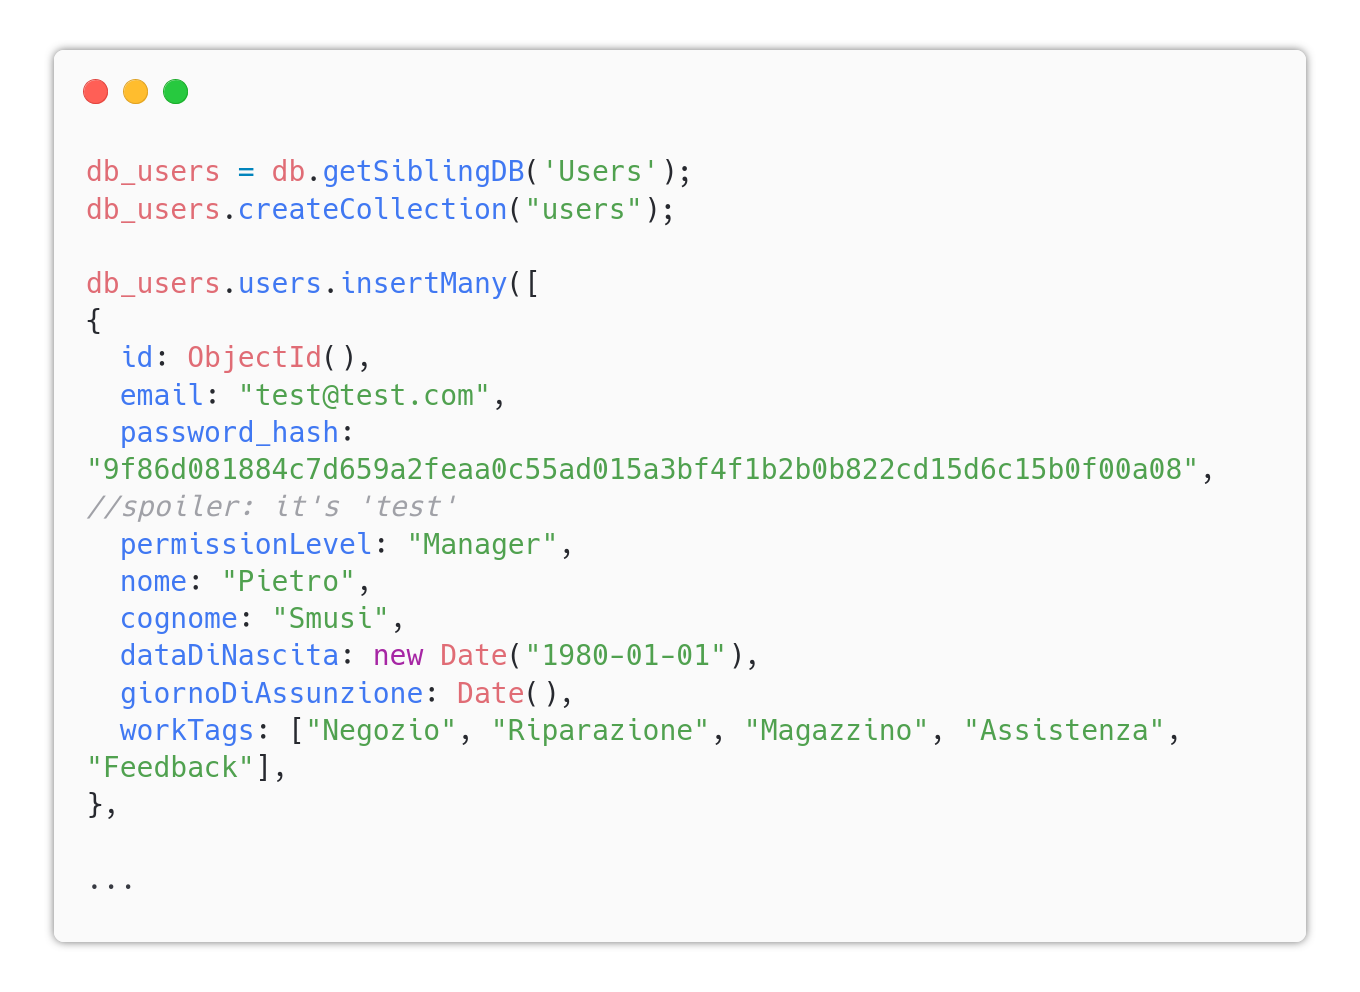
\includegraphics[width=1\textwidth]{images/db-users.png}
	Inizializzazione database "Users"
\end{figure}


\section{Parti comuni ad ogni microservizio}

In questa sezione verrà descritta la struttura che accomuna i vari microservizi.

\subsection{Scelta del Linguaggio}

Il linguaggio scelto per la backend e frontend è \textit{Typescript}: un linguaggio tipizzato che viene tradotto da un compilatore ("transpiler") in Javascript e dunque può essere eseguito in un web browser. Qualsiasi script JavaScript è anche codice TypeScript valido, questo permette all'applicazione di utilizzare l'ampia collezione di pacchetti JavaScript.

\subsection{Frameworks e Dipendenze}

Ogni microservizio utilizza:
\begin{itemize}
	\item \textit{ts-node} v10.9.2: ambiente runtime Typescript open source e multipiattaforma per la creazione del server di backend.
	\item \textit{eslint} v8.56.0: analizzatore di codice statico.
	\item \textit{nodemon} v3.0.3: tool di assistenza per Node.js. permette il riavvio automatico del server quando viene rilevata una modifica nel codice.
	\item \textit{express} v4.18.2: framework web per Node.js, utilizzato per la realizzazione di api.
	\item \textit{React} v18.3.0: libreria UI per javascript, utilizzata per la frontend.
	\item \textit{tailwindcss} v3.4.1: framework CSS.
	\item \textit{Jest} v29.7.0 : framework per il testing
	\item \textit{supertest} v7.0.0: framework per il testing di api, utilizzato insieme a Jest. 
	\item \textit{concurrently} v8.2.2: esegue più comandi contemporaneamente, utilizzato per eseguire frontend e backend insieme.
	\item \textit{serve} v14.2.3: hosta un sito statico, utilizzato per hostare la frontend in produzione.
	\item \textit{dotenv} v16.4.5: permette l'accesso alle variabili di ambiente, utilizzate per la configurazione dei microservizi.
	\item \textit{body-parser} v1.20.2: permette di leggere il body di una richiesta http.
	\item \textit{mongodb} v6.5.0: interfaccia per la connessione al microservizio database.
\end{itemize}

\subsection{Struttura}

La cartella di un microservizio presenta i seguenti files:
\begin{figure}[H]
	\centering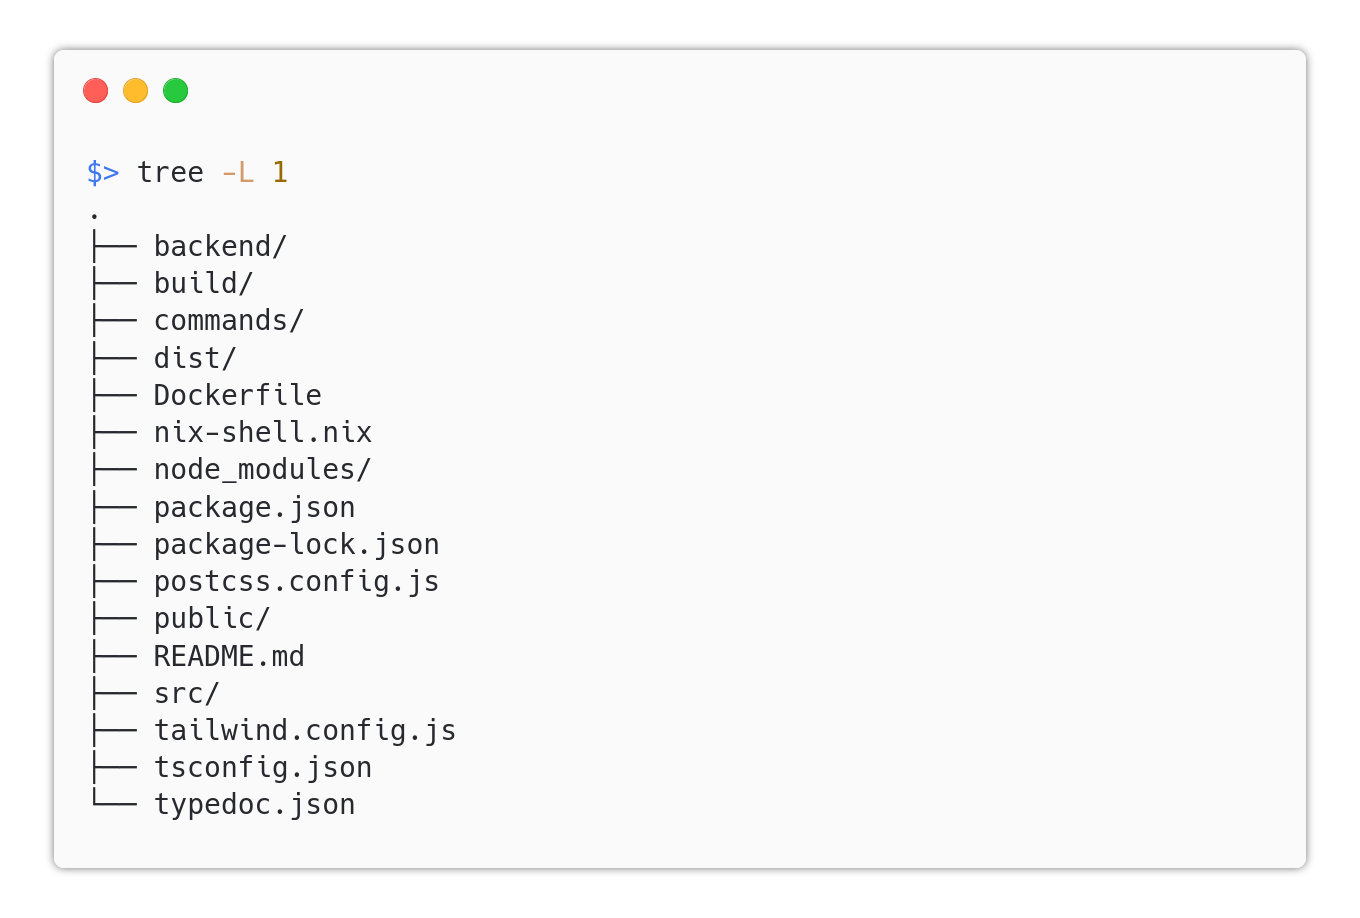
\includegraphics[width=1\textwidth]{images/structure.png}
	Output del comando "tree" all'interno di un microservizio.
\end{figure}
Segue una descrizione degli stessi, dall'alto verso il basso:
\begin{itemize}
	\item "backend": cartella contenente tutto il codice di Backend in TypeScript.
	\item "build": cartella contenente l'applicazione web statica generata da React.
	\item "commands": cartella contenente degli appunti degli sviluppatori durante la creazione del progetto.
	\item "dist": cartella contenente il codice backend per la produzione, generato dal compilatore di TypeScript.
	\item "Dockerfile": file contenente le istruzioni per la generazione del contenitore di docker.
	\item "nix-shell.nix": file contenente l'ambiente di sviluppo per chi sviluppa su NixOS.
	\item "node\_modules/": cartella contenente i moduli utilizzati dall'applicazione
	\item "package.json": file che definise le dipendenze e le impostazioni di vari moduli.
	\item "package-lock.json": contiene le versioni delle dipendenze dei moduli.
	\item "postcss.config.js": script di configurazione necessario per tailwindcss
	\item "public": contiene file di accesso pubblico per la frontned, come favicon.ico, robots.txt, index.html.
	\item "README.md": contiene le informazioni del progetto e le istruzioni per il deploy.
	\item "src/": cartella contenente tutto il codice per la frontend in tsx.
	\item "tailwind.config.js": file di configurazione per il funzionamento di tailwindcss
	\item "tsconfig.json": configurazione per TypeScript.
\end{itemize}

\subsection{Comandi npm}
Vengono definiti i seguenti scripts per l'esecuzione dell'applicazione tramite npm. Ogni comando può esssere eseguito digitando "npm run" ed il nome del comando.
\begin{itemize}
	\item "startfront": esegue solo la frontend, si aggiorna automaticamente ad ogni modifica del codice
	\item "buildfront": genera la frontend statica per la production
	\item "startback": esegue soltanto il server di backend, si aggiorna automaticamente ad ogni modifica del codice
	\item "start": esegue sia la frontend sia la backend in developement mode
	\item "production": esegue sia la frontend sia la backend in production mode
	\item "lint": esegue un'analisi stica del codice
	\item "test": esegue gli script di testing del codice.
\end{itemize}
	

\section{Microservizio Autenticazione}

\section{Microservizio Task}

\subsection*{Crea Task}

\subsection*{Modifica Stato Task}

\subsection*{Scegli Task}

\subsection*{Get Lista Task In Lavorazione}

\subsection*{Get Lista Task Da Eseguire}

\subsection*{Get Lista Task In Pausa}

\subsection*{Get Storico Task}

\subsection*{Testing routes}

\subsubsection*{Greet}
\subsubsection*{Test Task}
\subsubsection*{Test DB}

\section{Microservizio Gestione Dipendenti}

\section{Microservizio Home}

\chapter{Frontend}

	
\end{document}